\chapter{背景}
\label{background}

本章では本研究の背景について述べる。
まず機械学習における活性化関数のの役割について明確にする。
また、統計学において活性化関数に相当する概念がどのように応用されてきたか述べる。
活性化関数について概説し、現在の機械学習における活性化関数の抱える問題点を明らかにする。
次に、活性化関数の他に、ニューラルネットワークにおける精度を向上させるいくつかの構成要素について述べる。
本研究の問題点の解決に必要な、ノンパラメトリックモデルとその具体例であるカーネル密度推定を導入する。
最後に、実社会において機械学習を行う上での問題点や課題を述べる。



\section{活性化関数}

\begin{figure}[hbtp]
    \begin{center}
        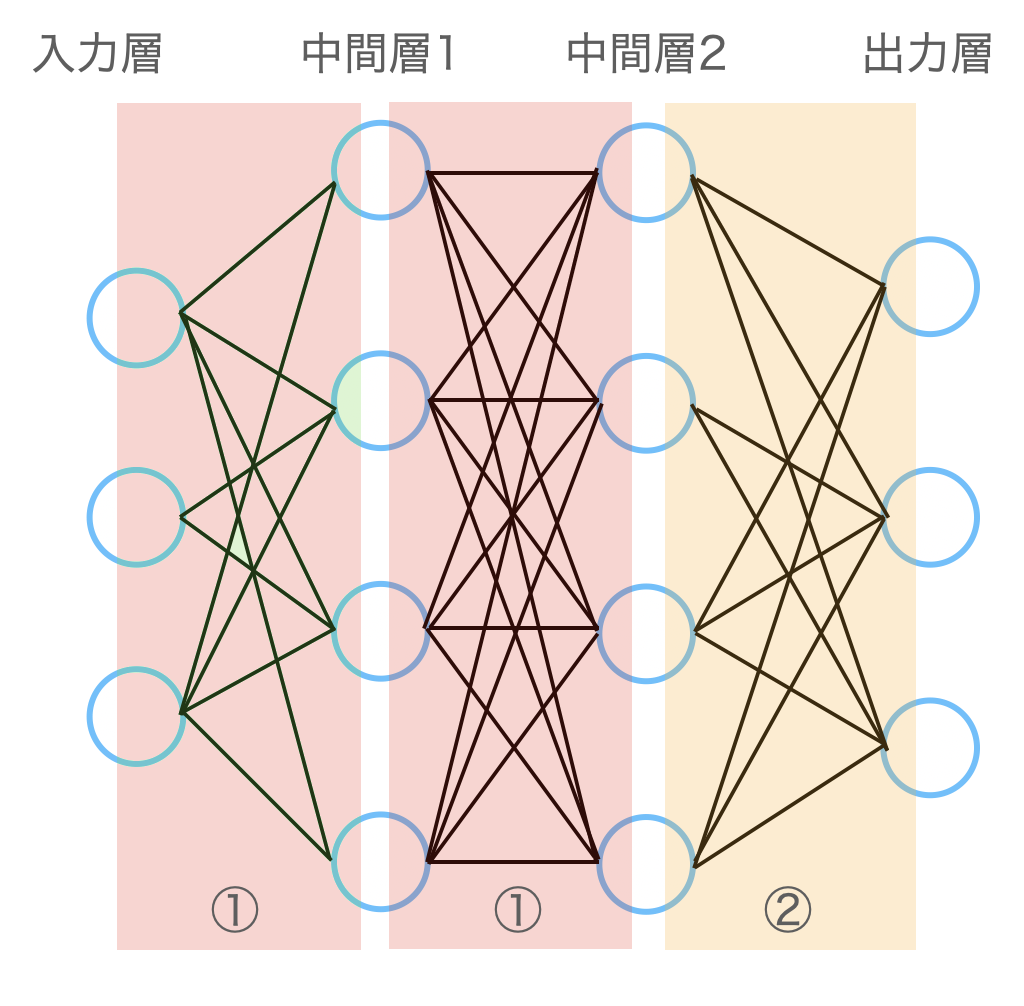
\includegraphics[width=10cm]{asset/neural_network2.png}
            \caption{活性化関数の領域。\textcircled{\scriptsize 1}、\textcircled{\scriptsize 2}の領域によって使われる活性化関数が変わることが多い。}
            \label{neural_network1}
    \end{center}
\end{figure}

また、概要を述べるにあたってニューラルネットワークの用語を定義する。活性化関数は
図\ref{neural_network1}の\textcircled{\scriptsize 1}の部分で使用する活性化関数を「中間層の活性化関数」、\textcircled{\scriptsize 2}の部分で使用する活性化関数を「中間層の活性化関数」と記述することとする。

ディープラーニングの活性化関数に関する最近の研究はまだ多く、様々な実験が 行われている~\cite{study_af}。
活性化関数の歴史はSigmoidという統計学的にも馴染み深いロジスティック回帰のモデルから始まった。
ニューラルネットワークの層に活性化関数を適用する過程を以下に示す。
$ w_i$ を重み、$ \mathbf{X}_i $ は入力の値、$ b $はバイアス、$z$ は出力、$ g $ を活性化関数とした時
$ z=g(y)=g(\sum w_i \mathbf{X}_i+b) $ 
このように用いられる。
その後TanhやXavierのReLU(2011)~\cite{ReLU}などといったより計算に適した活性化関数が発見されてきた。
特にReLUに関しては現在のディープラーニングなどの深層ニューラルネットワークにおいても未だ応用されており、実用的にもその有用性が示されていることがわかる。

長年にわたり、性能を向上させ、ReLUの欠点に対処する多くの活性化関数が提案されてきたが、その中にはLeaky ReLU ~\cite{leaky_relu}、ELU~\cite{elu}、SELU~\cite{selu}などが含まれる。
Prajit RamachandranのSwish(2017)~\cite{swish}は、$ f(x)=x {\bf sigmoid}(\beta x) $ と定義できるが、よりロバストな活性化関数であることが証明され、ReLUと比較して結果が大幅に改善された。
活性化関数はそれまで単調増加な関数が使われることが多かったが、Swishで単調増加である必要なく、汎用的に精度が向上することがわかった。
またそのような活性化関数の例としてDiganta. MisraのMish(2019)~\cite{Mish}と言う活性化関数も提唱されている。

\begin{table}[htbp]
    \begin{center}
        \caption{活性化関数の種類}
        \vspace{2mm} 
        \label{|class_af|}
        \begin{tabular}{|cp{5cm}cc|}
        \hline
        活性化関数の式              & 式 & & \\
        \hline
        Sigmoid            & $ \cfrac{1}{1 + \mathrm{exp}(x)} $ & & \\
        \hline
        Tanh               & tanh(x) & &  \\
        \hline
        \multirow{5}{*}{ReLU}        &  \[{\rm output} =
            \begin{cases} 
            0 &\text{when $ x < 0 $ }\\
            x &\text{when $ x \geq 0 $ else} \\
            \end{cases}
            \] & & \\
        \hline
        Swish           & $ x\cdot {\rm sigmoid}(\beta x) $ & & \\
        \hline
        Mish           & $ x\cdot {\rm tanh}(\log (1 + \mathrm{exp}(x) )) $ & &  \\
        \hline

        \end{tabular}
    \end{center}
\end{table}



\begin{eqnarray}
\dot g = \frac{M}{\|g\|} g
\label{eq:hassan}
\end{eqnarray}




\section{統計学における位置付け}

\begin{figure}[hbtp]
        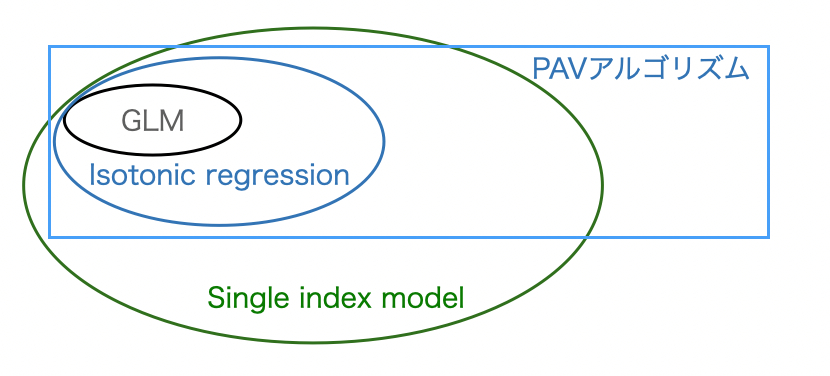
\includegraphics[width=15cm]{asset/machine_statistics.png}
            \caption{機械学習と統計学の繋がり}
            \label{glm}
\end{figure}

活性化関数の概念は統計学におけるリンク関数と呼ばれるモデルの汎用性を高める動きに始まり、機械学習へと応用されている。
本項目ではその理解に必要な知識を述べていく。



\subsection{一般化線形モデルとは}


\begin{figure}[hbtp]
        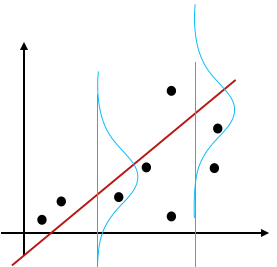
\includegraphics[width=6cm]{asset/glm1.png}~~~~~ ~~~~~ 
        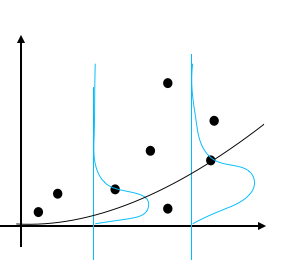
\includegraphics[width=6cm]{asset/glm2.png}
            \caption{一般化線形モデルの必要性}
            \label{glm}
\end{figure}

説明変数を$ X $, パラメータを$ W $で表現し、従属変数を$ Y $、誤差を$ \epsilon \sim \mathcal{G}(0, \sigma^2) $で表現すると、一般線形モデルは以下の式で表現することができる。

\begin{eqnarray}
\mathbf{Y} = \mathbf{X} \cdot  \mathbf{W} + \epsilon
\label{eq:senkei}
\end{eqnarray}
またこれは$ \mathbf{Y} $の期待値を使って表現すると上記は
\begin{eqnarray}
    \mathrm{E}[\mathbf{Y}] &=& \mathrm{E}[\mathbf{X} \cdot  \mathbf{W} + \epsilon] \\
    \mathrm{E}[\mathbf{Y}] &=& \mathrm{E}[\mathbf{X} \cdot  \mathbf{W}] + \mathrm{E}[\epsilon] \\
    \mathrm{E}[\mathbf{Y}] &=& \mathbf{X} \cdot  \mathbf{W}
\label{eq:link}
\end{eqnarray}
である。
しかしながら、上記の式の展開では実際は図\ref{glm}左のように$ \epsilon $が正規分布に従うことを想定した、すなわち従属変数$ Y $がガウス分布に従うことを仮定したが、実際は図\ref{glm}右のように、誤差の分布にガウス分布を仮定すると、正確さが失われることがある。
そこで、従属変数をある関数 $ G $ で変換してからモデル化することでモデルの正確さが向上する。
すなわち、$ \mathrm{E}[\mathbf{Y|X}] = \mathbf{X} \cdot  \mathbf{W} $ に対して$ G(\mathrm{E}[Y|X]) = \mathbf{X} \cdot  \mathbf{W} $ となるような$ G $ を取り入流。
またこの$ G $ の逆関数 $ G^{-1} $をリンク関数と呼ぶ。
一般線形モデルに対して、リンク関数を加えた式を以下に記す。
\begin{eqnarray}
\mathrm{E}[\mathbf{Y|X}]=G^{-1} (\mathbf{X}\cdot  \mathbf{W})
\label{eq:link}
\end{eqnarray}

一般に誤差構造が決まれば、リンク関数も自動的に決まる。
ガウス分布の場合のリンク関数は$ G(U) = U $である。
これらの結果は$ G^{-1} $を単調増加な任意の関数に置き換えることでさまざまなモデルを表現することが可能になる。


\subsection{Sigmoid関数とロジスティック回帰}
\label{history_sigmoid}
\begin{eqnarray}
G(\mathbf{Y})=\mathbf{X}\cdot  \mathbf{W}
\end{eqnarray}
とした時、
\begin{eqnarray}
G=\log \bigl(\frac{y}{1-y}\bigr)
\end{eqnarray}
とする。一般的にこれはロジット関数と呼ばれる。
これを左辺が$ y $になるように変形すると,

\begin{eqnarray}
\log \bigl(\frac{y}{1-y}\bigr) = z \\
y = \frac{1}{1 + \exp(-z)}
\end{eqnarray}
右辺を$ z $を関数にすると

\begin{eqnarray}
g(z) = \frac{1}{1 + \exp(-z)}
\end{eqnarray}
となり、これはSigmoid関数である。
$ g(z) $はロジスティック関数でもあり、


\begin{eqnarray}
y = \frac{1}{1 + \exp (\mathbf{X} \cdot  \mathbf{W})}
\end{eqnarray}
より、ロジスティック回帰であることも示される。 \\

これらにより、ニューラルネットワークに出てくるSigmoid関数が潜在的に統計学の世界でも出てくることがわかる。






\begin{figure}[hbtp]
    \begin{center}
        \begin{tabular}{c}
            \begin{minipage}{0.40\hsize}
                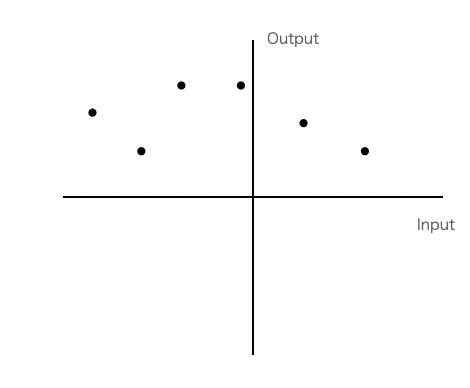
\includegraphics[clip, width=5cm]{asset/k_af_band1.png}
                    \caption{カーネル密度推定に用いるデータ点の集合}
                    \label{k_af_band1}
            \end{minipage}
            \hspace{10pt}
            \begin{minipage}{0.40\hsize}
                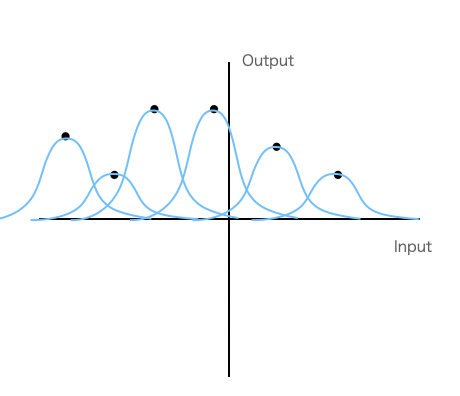
\includegraphics[clip, width=5cm]{asset/k_af_band2.png}
                    \caption{カーネル関数、今回はガウス関数でその周辺ごと近似する。}
                    \label{k_af_band2}
            \end{minipage}
            \hspace{10pt} \\
            \vspace{10pt} \\
            \begin{minipage}{0.40\hsize}
                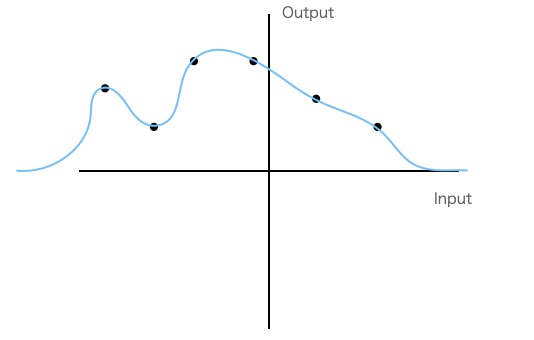
\includegraphics[clip, width=5cm]{asset/k_af_band3.png}
                    \caption{点の周辺のカーネル関数を足し合わせた時にできる関数}
                    \label{k_af_band3}
            \end{minipage}
        \end{tabular}
    \end{center}
\end{figure}


\subsection{ノンパラメトリックとカーネル密度推定}
統計学において、パラメータで表現されるモデルや確率分布を使用すものをパラメトリックな手法として分類するが、パラメータを使用せずモデルを表現する手法をノンパラメトリック手法という。
ノンパラメトリックを代表する手法の一つにカーネル密度推定と呼ばれる手法がある~\cite{kernel_density}。
これは、ある母集団のデータが与えられたとき、カーネル関数を用いてその関数を推定する手法である。
カーネル関数とは、与えられた領域内で積分した時に1となり、対称性を持つものとしてイメージして良い。
カーネル関数の代表例としてガウス関数があげられる。

$ K $をカーネル関数 $ u \in \reals $ とした時、カーネル関数の定義は以下である。

\begin{itemize}
  \item $ \int^{+ \infty}_{- \infty} K(u)du = 1 $
  \item $ K(-u) = K(u) $
\end{itemize}


この時、カーネル密度推定法とは、$ \mathbf{X}_n $をデータ、推定すべき関数を$ f $、カーネル関数を $ K $、バンド幅を $ h $ としたとき、以下の式で表現することができる。


\begin{eqnarray}
f(x) = \frac{1}{nh} \sum^n_{i=1}K \bigl( \frac{x - \mathbf{X}_i}{h}\bigr)
\label{eq:k-af}
\end{eqnarray}
図\ref{k_af_band1}のようにまばらに存在するデータ点の周辺に、図\ref{k_af_band2}のようにカーネル関数をおき、任意のバンド幅で足し合わせ近似していくようなものである。






\subsection{セミパラメトリックモデルとSingleIndexModel}

統計学の世界では、セミパラメトリックモデルというノンパラメトリックな手法とセミパラメトリックな手法を組み合わせた手法が存在する。
その中の一つの代表的な手法の中にSingleIndexModel(SIM)と呼ばれる手法が存在する。
SIMとは、未知の関数 $ g $、従属変数 $ Y $、説明変数$ X $、パラメータ$ W $、誤差項 $ \epsilon $と置いた時、以下のように表される式である。

\begin{eqnarray}
Y = g(\mathbf{X} \cdot  \mathbf{W}) + \epsilon
\label{eq:k-af}
\end{eqnarray}

SIMは未知の関数$ g $を推定しながらパラメータ $ W $を求めていく問題に帰着されるため、ノンパラメトリックとパラメトリックが混ざった手法であるセミパラメトリックモデルとして表現される理由である。
この$ g $は、一般化線形モデルのリンク関数$ G^{-1} $ をさらに一般化した単調増加性を無くしたモデルだと考えることができる。
SIMの有名なモデルの一つにisotonic regressionと呼ばれるものがある。

\begin{figure}[hbtp]

    \begin{center}
        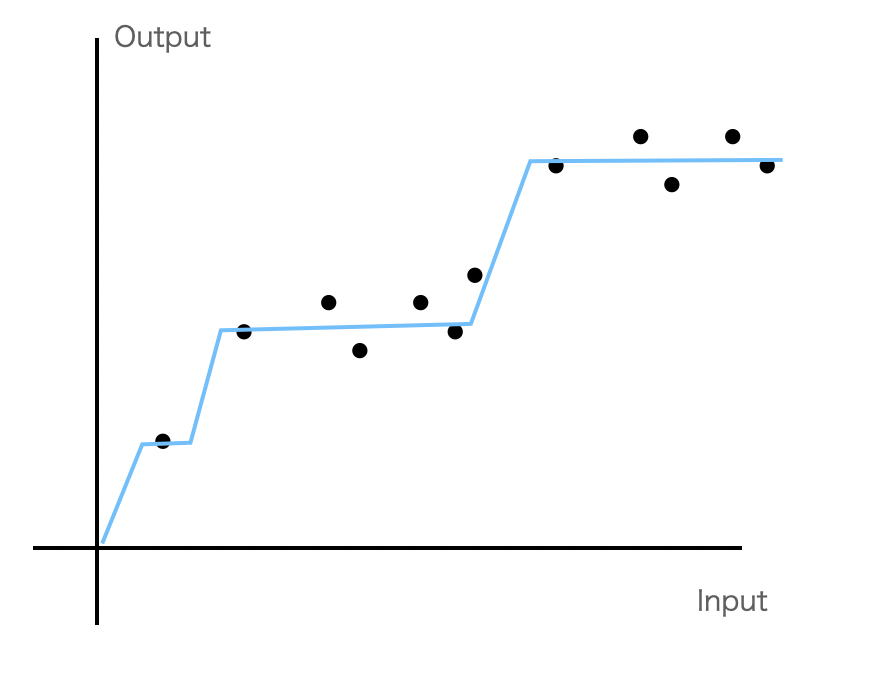
\includegraphics[width=10cm]{asset/isotonic_regression.png}
            \caption{SingleIndexModelの例の一つのisotonic regression}
            \label{isotonic_regression}
    \end{center}
\end{figure}

isotonic regressionは単調増加性等の制約を仮定したSIMの一つで、化学分野や経済分野に応用されている。


\subsection {セミパラメトリックモデルと機械学習学習}

セミパラメトリックにモデルを推定する手法は統計学ではIchimura(1993)~\cite{ichimura}から始まり、PAVアルゴリズムとしてAdam Tauman Kalai(2008)~\cite{isotron}によりその有用性が確かめられた。

\subsubsection{Ichimuraの手法}

SIMの未知の関数をleave one out法を用いたカーネル密度推定法と最尤推定により導く試みはIchimura(1993)~\cite{ichimura}や Klein(1993)~\cite{klein}によって提案され始めた。

Ichimura(1993)の手法はSingleIndexModelのノンパラメトリック関数を以下の式で近似する手法である。


\begin{eqnarray}
G(\mathbf{X}_iw)=\frac{\sum_{i\neq j} K\left(\frac{\mathbf{X}_j w - \mathbf{X}_i w}{h}\right)\mathbf{Y}_j}{\sum_{i\neq j} K\left(\frac{\mathbf{X}_j w - \mathbf{X}_i w}{h}\right)}
\label{eq:ichimura}
\end{eqnarray}

ここで、$ K $はカーネル関数である。$ i \neq j $ とすることにより、$ \mathbf{X}_i $を入力した時の値が$ y_i $へと過剰適合しないようにするためである。



\subsubsection{PAVアルゴリズム}

SIMやisotonic regressionを機械学習に応用する試みはAdam Tauman Kalai~\cite{isotron}のPAVアルゴリズムと呼ばれる手法で、分類問題の応用へと繋がった。
isotonic regression自体は回帰問題として発明された手法であったが、これによりアルゴリズム的に分類問題がセミパラメトリックな手法を用いて解くことが可能であることが発見された。
この手法をベースにSham Kakade(2011)~\cite{efficient_sim}やRavi Ganti(2015)~\cite{lsim}などによってより高速で汎用的なisotonic regressionを応用したセミパラメトリックモデルの分類問題の解法のアルゴリズムが導かれた。


\section{勾配法と学習における知識}
機械学習の問題の多くは学習の際の最適なパラメータを探索する。最適なパラメータとは損失関数が最小値を撮る時の値のことである。
勾配法とは関数の勾配方向に閾値を移動させることで、関数の最小値を見つける方法のことである。特にニューラルネットにおいては最小値を見つけるために、勾配法がよく用いられる。
損失関数を$ E $, $ w_i $をiステップ目のパラメータとした時、勾配法を式で表すと以下のようになる。

\begin{eqnarray}
w_{i + 1} = w_i - \mu \frac{\partial E}{\partial w}
\label{eq:learning_rate}
\end{eqnarray}

複雑な損失関数を最小化させるためのテクニカルな手法として、学習率、初期パラメータ、正則化などと言ったものが挙げられる。
本項ではこれらについて必要な概念を述べる。
\subsection{LearningRate(学習率)}

LearningRateとはハイパーパラメータの一つで、式(\ref{eq:learning_rate})の$ \mu $に相当する部分である。
LearningRateは大きいほど収束の可能性は小さくなり、小さいほど学習が遅くなる。
また、高いLearningRateでも安定して学習できる活性化関数が求められている。


\subsection{Initializer(重みの初期化)}
ニューラルネットワークの学習効率は、重みの初期値によって大きく変わることが知られている。
例えば初期値を全て$ 0 $に固定すると、逆誤差伝播の影響で重みが均一になることにより、重みを多く持つ意味がなくなる。
この問題を解消するために、学習のテクニックとして以下のような手法がある。
また、重みの初期化手法を総称してInitializerと記述する。

\subsubsection{Xavier initializer}
Xavier(2010)~\cite{xavier}によって提唱された重みの初期化手法の一つで、現在最もニューラルネットワークの学習で利用されてる手法である。
ニューラルネットワークの$ i $層の重みの数を$ n_{i} $、重みを$ w_i $、一様分布を$U$ で表現した時

\begin{eqnarray}
w_{i} \sim U \bigl[ - \frac{\sqrt{6}}{ \sqrt{n_i + n_{i+1}} }, \frac{\sqrt{6}}{ \sqrt{n_i + n_{i+1} }} \bigr]
\end{eqnarray}
で初期化する手法である。これにより初期化すると、重みの分布が広がりを持つことが知られている。
活性化関数がLinear、Sigmoid、Tanhの時に有効に働く。

\subsubsection{KaimingUniform}
Kaiming He(2015)~\cite{kaiming}によって提案された初期化の手法で、以下の分布から重みをサンプリングする。

\begin{eqnarray}
w_{i} \sim U \bigl[ - \frac{\sqrt{6}}{ \sqrt{n_{i+1}} }, \frac{\sqrt{6}}{ \sqrt{ n_{i+1} }} \bigr]
\end{eqnarray}

主にReLUに有効になる。


\subsection{Regularizer(正則化)}
ニューラルネットワークは訓練データを過剰に学習すると未知データへの予測精度が落ちることがある。
これはモデルが訓練データに対して過剰に学習したために、はずれ値やノイズまで学習してしまうことに起因する問題である。
このような現象を過学習というが、この過学習を防ぐためにパラメータに対して一種の罰則をかけるようなことが一般的に行われている。

損失関数を$ E(w) $とした時に、最適化する関数を$E(w)$の代わりに以下の式を用いる。

\begin{eqnarray}
E(w) + \lambda \frac{1}{p}\|w\|^p_p
\label{eq:regu}
\end{eqnarray}


ここで$ w $はパラメータベクトルで$ \| \cdot \| $はL1ノルム(p=1)やL2ノルム(p=2)などである。$ \lambda $ はハイパーパラメータである。


\begin{figure}[hbtp]
    \begin{center}
        \begin{tabular}{c}
            \begin{minipage}{0.40\hsize}
                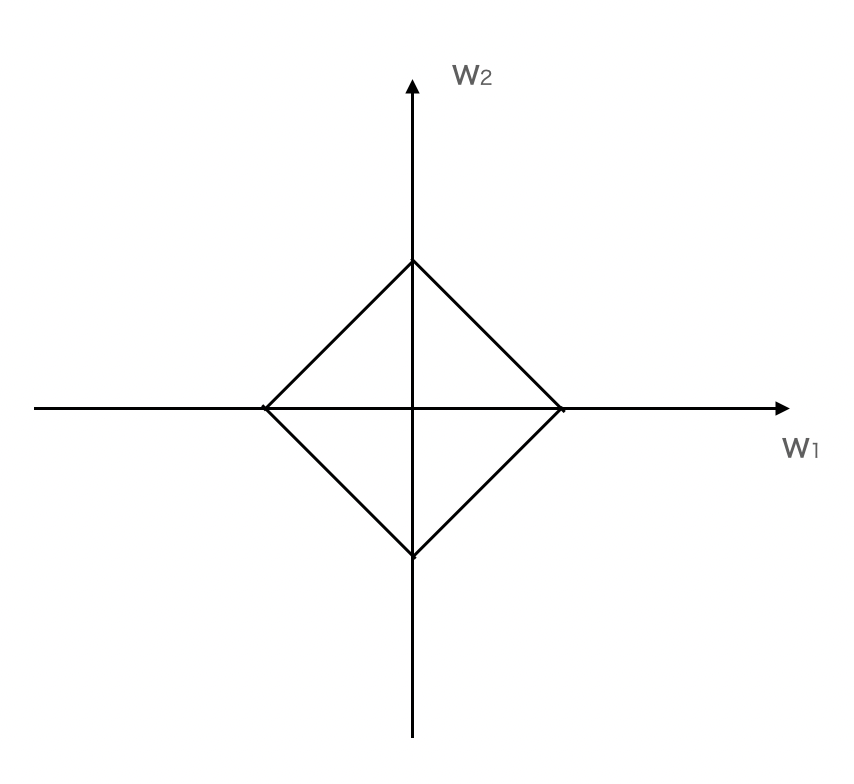
\includegraphics[clip, width=5cm]{asset/l1norm.png}
                    \caption{パラメータが二つの時のL2ノルムのイメージ図。パラメータが二つある時、その合計値($ \sum_i w_i $)が$ 1 $の点を取ると、一つのパラメータを$ 0 $にすることが最も大きくなる。}
                    \label{l1norm}
            \end{minipage}
            \hspace{10pt}
            \begin{minipage}{0.40\hsize}
                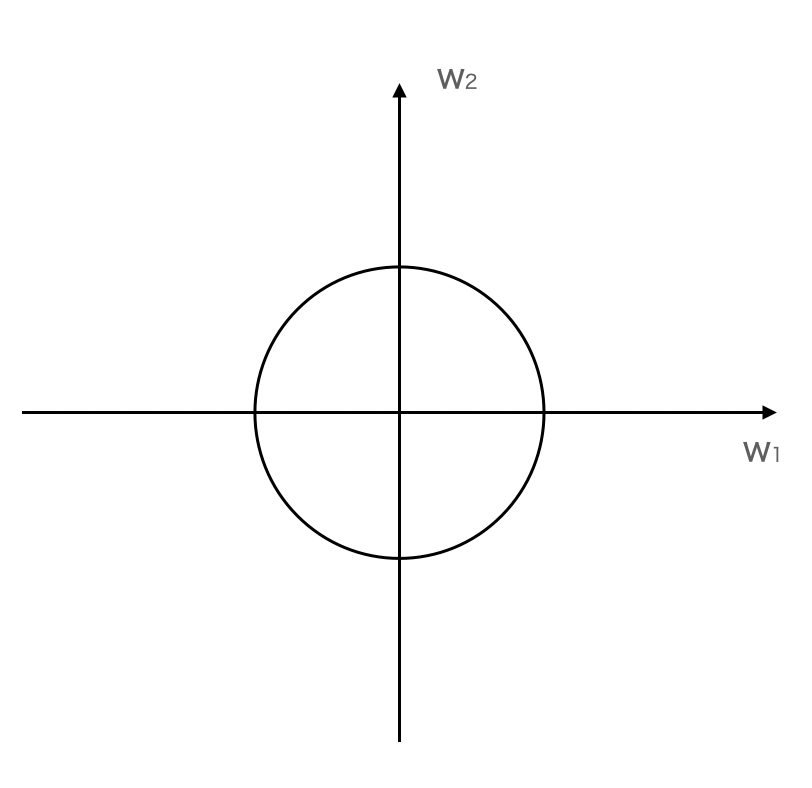
\includegraphics[clip, width=5cm]{asset/l2norm.png}
                    \caption{パラメータが二つの時のL2ノルムのイメージ図。パラメータの合計値その合計値($ \sum_i w_i $)が$ 1 $の時は$ w_1 = w_2 = 0.5 $の時が最も値が小さくなるので、より高次元で考えるとこの値を大きくするのは均一的な重み分布であることが望ましい。}
                    \label{l2norm}
            \end{minipage}
        \end{tabular}
    \end{center}
\end{figure}




\subsubsection{L1ノルム}
L1正則化は余分なパラメータ(説明変数)を省くことを目的とした手法である。
\ref{eq:regu}の式を考えると、モデルに必要ないパラメータを$ 0 $にすることが損失関数の最小化につながることがわかる。
この結果は、主に次元の圧縮などに対して応用することも可能である。

\subsubsection{L2ノルム}
L2ノルムの値を$ L2 $、L1ノルムの値を$ L1 $、またパラメータの合計値($ \sum_i w_i $)が等しい場合においては

\begin{eqnarray}
L2 < L1
\label{eq:norm uneq}
\end{eqnarray}
であることがわかる。これはL1ノルム同様に一つのパラメータを$ 0 $に対することの影響度が関数全体に対して小さいことを表していると考えられる。
以上によりL2ノルムの最小化は、均一的にパラメータを小さくすることで、最小化を図ることができる。
以上によりL2ノルムの罰則を足した合わせた損失関数により最小化したニューラルネットワークはパラメータ数が多いため、"表現力に優れている"と表現することが可能である。
これは過学習の回避に用いることができる。


\subsection{データセットの選択}
ニューラルネットワークの最適化の際に学習データセットをどのように用いるかによって性能が大きく変わることが知られている。
データセットの集合を$ \mathcal{D} $ 大きく分けて以下の三つの方法があることが知られている。

\begin{table}[htbp]
    \begin{center}
        \caption{実験に用いるデータ集合の表現方法}
        \vspace{2mm} 
        \begin{tabular}{|c|c|c|}
        \hline
        扱うデータ      & 名称 & 説明 \\
        \hline
        $ \mathcal{D}_i \subseteq \mathcal{D} $          & ミニバッチ学習  & データを部分的にランダムで取り出して学習を行う \\
        \hline
        $ d_i \in \mathcal{D} $                & オンライン学習 & データを一つ取り出して学習を行う  \\
        \hline
        $ \mathcal{D}  $      & バッチ学習 & 全てのデータを用いて学習する \\
        \hline
        \end{tabular}
    \end{center}
\end{table}

バッチ学習は安定した学習が行える一方で欠点は大きく以下の二つがある。

\begin{itemize}
  \item 損失関数の形が変わらないため、最適化の手法によっては学習が停滞してしまう。
  \item データ数が大きい場合には損失関数が大きくなり、メモリ不足等の問題が発生する。
\end{itemize}

また、オンライン学習は局所界に陥りにくいというメリットがあるものの、以下欠点が存在する。

\begin{itemize}
  \item 最初より最後のデータに過剰に適合してしまう。
  \item 外れ値にも反応しやすいため、パラメータの収束が不安定になる。
\end{itemize}

以上により一般的に両者の欠点を抑えたミニバッチ学習が実務では使用されることが多い。

\subsection{Optimizer}
ニューラルネットワークの学習の目的は、損失関すの値をできるだけ小さくするパラメータを見つけることである。
これは最適なパラメータを見つける問題であり、その問題を解くことを最適化という。

\ref{eq:learning_rate}で表現した手法も最適化の一つである。
これは確率的勾配効果法(SGD)と言って単純な方法であるが、パラメータ空間を闇雲に探すよりは遥かに効率的な方法である。
しかしながら、SGD以外にもパラメータをよりよく最適化する方法は多く研究されている。

\subsubsection{SGD}
SGDは(\ref{eq:learning_rate})でも記したように以下の式の形で一般的に広く知れ渡り、実装が簡単な手法として認知されている。

\begin{eqnarray}
\mathrm{W} \leftarrow \mathrm{W} - \mu \frac{\partial E}{\partial \mathrm{W}} \\
\label{eq:sgd}
\end{eqnarray}

ここで、$ \mathrm{W} $ は各パラメータ $ w_i $をベクトルで表現したものである。

しかしながら式からもわかるようにSGDには欠点とした以下の二つが広く認知されている。




\begin{itemize}
  \item 勾配が0の点では学習が進まなくなる。
  \item 勾配の方向が本来の最小値の方向を指していないことがある。
\end{itemize}
これらの理由により近年では実用的には使用されていない。

\subsubsection{Momentum}

Ning QianのMomentum(1999)~\cite{momentum}はSGDの勾配の方向が本来の最小値ではないという考えから、物理の法則を応用するような形で生まれた勾配法の一つである。


Momentum という手法は、式で次のように表される。

\begin{eqnarray}
    \mathrm{v} \leftarrow \alpha \mathrm{v} - \mu \frac {\partial E }{\partial \mathrm{W}} \\
    \mathrm{W} \leftarrow \mathrm{W+v}
\label{eq:momentum}
\end{eqnarray}

ここで新しく$ \mathrm{v} $という変数が登場する。これは一つ前の勾配の速度のようなものを記録しており、勾配が急なところでは大きな値になり、小さなところでは値が小さくなる。
これによりSGDに比べると更新するときの"ジグザグ度合い"のようなものが軽減され、学習が安定し高速化することが知られている。


\subsubsection{AdaGrad}

ニューラルネットワークの学習では学習係数の値が重要になる。
これを初めは大きく学習し、次第に小さ学習する、学習係数の減衰(learning rate decay)という方法がよく使われる。
これを発展させた方法にJohn DuchiのAdaGrad(2011)~\cite{adagrad}というものがある。
AdaGradは以下の式で表現できる。

\begin{eqnarray} 
    \mathrm{h} \leftarrow \alpha \mathrm{h} + \frac {\partial E }{\partial \mathrm{W}} \odot \frac {\partial E }{\partial \mathrm{W}}  \\
    \mathrm{W} \leftarrow \mathrm{W}  - \mu \frac{ 1 }{\sqrt{\mathrm{h}}} \frac{ \partial E }{\partial \mathrm{W}} 
\label{eq:adagrad}
\end{eqnarray}

ここで$ \odot $は行列の要素ごとの掛け算を意味する。パラメータ更新の際に$ \frac{ 1 }{\sqrt{\mathrm{h}}} $を乗算することで、学習スケールを調整するという手法である。
これにより、よく動いた学習パラメータは次第に小さくなる。



\subsubsection{Adam}
物理的なテクニックを応用するMomentumと学習係数を調整するAdaGradを掛け合わせたせるのがDiederik P. Kingma(2014)~\cite{adam} である。
機械学習の世界では最も頻繁に用いられる。


\subsection{勾配爆発問題}
勾配爆発問題とは、ニューラルネットワークの設計において、勾配が発散することで学習が進まなくなる技術的な問題のことである。
勾配発散の問題はRNN~\cite{rnn}などの行列の積が絡む問題やGAN~\cite{gan}などの誤差関数が不連続のな場合では簡単に発生する問題である。
これを対処するためには簡単な手法としてパラメータの勾配の上限値を決めるクリッピングという操作を用いる方法などが挙げられる。
勾配を$ g $、勾配の上限値を$ M $で表現した場合に、勾配を以下式(\ref{eq:hassan})のように変換する。



\section{実社会における学習の問題点}

ディープラーニングをGUIで簡易的に扱えるツールは様々な企業が積極的に開発しており、50以上のツールがあることが確認されている~\cite{gui}。
しかしながらこれらのツールの共通として存在する問題点は画像分類に強いなどといった特化型となっており、それぞれの問題に応じて使い分ける必要が出てくるということである。
機械学習では問題は大きく分けて回帰と分類の二つが存在するが、初学者にはそのような問題に応じたモデルの構築や学習を各ツールと状況に応じて使い分けることは非常に困難である。
このような点からコスト的面でも、初学者向けのツールであってもデータセットの形や目的を意識せずとも利用できるような学習アルゴリズムが求められている。


\section{汎用的な活性化関数}

ReLUやSwish, Mishといった活性化関数は、どれも実験的に精度が向上すると言う理由で選択されたものである。
そのため、あらゆるパターンにおいて最適かどうかは未知数である。
このような問題を解決するため、Alberto Marchisio(2018)~\cite{automatic_af}が提唱した手法では、既存の活性化関数の中から最適なもの見出し精度を向上させる方法を提唱した。
しかし、この方法にも欠点があり既知の活性化関数が問題に応じた適切な活性化関数かどうか判断する方法は存在しない。
Garrett Bingham(2020)~\cite{evo_af}は進化的アルゴリズムを用いて$ x^2 $や $ \sin (x) $といった原始的関数を組み合わせ最適な活性化関数を見つけることが提唱されている。
しかしこの方法は、計算量が重く、関数全体の空間を探査できるかどうかは原始的関数の組み合わせに依存してしまう。




